\documentclass[11pt]{article}

\usepackage[margin=1in]{geometry}
\usepackage[T1]{fontenc}
\usepackage[utf8]{inputenc}
\usepackage{lmodern}
\usepackage{microtype}
\usepackage{amsmath, amssymb, amsfonts}
\usepackage{bm}
\usepackage{graphicx}
\usepackage{booktabs}
\usepackage{multirow}
\usepackage{xcolor}
\usepackage{hyperref}
\usepackage[nameinlink,capitalise]{cleveref}
\usepackage{enumitem}

\hypersetup{
  colorlinks=true,
  linkcolor=blue!50!black,
  citecolor=blue!50!black,
  urlcolor=blue!50!black
}

\title{Layer-Depth Attention Routing in Transformers}
\author{
Fan Shun\\
\texttt{fanshun@stu.scu.edu.cn}
\and
Hu Chaolang\thanks{Corresponding author: \texttt{huchaolang@scu.edu.cn}}\\
\texttt{huchaolang@scu.edu.cn}
}
\date{}

\begin{document}
\maketitle

\begin{abstract}
Transformers propagate information effectively along the token dimension, but access to same-position representations formed at earlier layers remains indirect. We study whether a token at the current layer can benefit from directly reading its own depth history, rather than relying only on repeated residual propagation through the stack. To this end, we introduce a layer-depth attention routing mechanism that augments standard self-attention with a same-position cross-layer memory branch. In this paper, we instantiate and evaluate this idea in decoder-only language models. The current implementation uses a single shared query for row-wise token attention and depth-wise memory retrieval, and archives one projected historical K/V entry per block. On WikiText-103, across multiple settings including 8-layer and 16-layer models, different sequence lengths, and long training budgets, the method improves final test perplexity over strong Transformer baselines by 1.3\% to 3.1\%. 
% Attention-allocation analyses further show that deeper layers assign substantial mass to the depth branch and selectively retrieve a small number of high-value early-layer memory slots, rather than ignoring the added pathway. Taken together, these results suggest that explicit depth history is a useful information source even for already strong decoder baselines, while also revealing a clear trade-off: the current prototype incurs noticeable runtime overhead.
Attention-allocation analyses further show that deeper layers assign substantial mass to the depth branch and selectively retrieve a small number of high-value early-layer memory slots, rather than ignoring the added pathway. Moreover, the relative allocation between the row and depth branches remains broadly stable across token positions, suggesting that the added depth pathway does not fade away as the token sequence becomes longer.


\end{abstract}

\section{Introduction}

Transformer language models are built around token-wise attention, where each layer reads contextual information from other positions in the sequence \cite{vaswani2017attention}. A useful way to interpret this architecture is as a two-dimensional computation graph over token positions and layer depth \cite{zhang2026residual}. Under this view, recurrent models mainly propagate information through chained local transitions, while self-attention sharply shortens communication along the token axis by allowing a token to access its prefix within one layer \cite{vaswani2017attention}. However, the same perspective also highlights a remaining asymmetry: representations formed by the same token at earlier layers are still only indirectly accessible in standard decoder-only Transformers.

Residual connections do provide a depth-wise transmission path, so standard Transformers are not entirely lacking in cross-layer communication \cite{he2016deep}. But this path is uniform and additive rather than selective: earlier-layer information is mixed forward through the residual stream, not explicitly retrieved on demand for the current token. As depth increases, useful earlier-layer signals may therefore be diluted among many subsequent transformations \cite{ravula2021realformer,kimi2026attnres,denseformer2024,dca2025,muddformer2025}. This motivates a simple question: can a decoder-only language model improve by augmenting token attention with a direct layer-depth memory branch? If the current token could jointly attend to both the usual row-wise prefix context and its own cross-layer history, then the model might reuse partially refined intermediate states more effectively instead of repeatedly reconstructing them through the stack.

This question is related to, but distinct from, several existing directions. On one side, long-context and recurrent-memory approaches such as Transformer-XL expand the usable temporal horizon by carrying information across segments \cite{dai2019transformerxl}. On another side, models such as Universal Transformer revisit how repeated computation can be organized across depth \cite{dehghani2018universal}, while parameter-sharing models such as ALBERT show that depth and parameterization need not be tied in a naive one-layer-one-parameter manner \cite{lan2019albert}. Our setting is narrower than both: we do not attempt to redesign the whole recurrence structure or compress parameters across depth, but instead expose a direct same-position retrieval path inside an otherwise standard decoder stack.

In this work, we study this question through a controlled family of cross-layer memory mechanisms for decoder-only Transformers. Our current design uses a single query to route both row-wise token attention and depth-wise memory retrieval, and archives one projected historical K/V entry per block. The resulting mechanism extends each attention step from pure token interaction to a joint token-depth routing problem. In the computation-graph view, the method preserves the short communication path along the token axis while introducing a more direct access path along the depth axis.

The resulting gains are not dramatic, but they are stable. Across multiple WikiText-103 settings, including 8-layer and 16-layer models, different sequence lengths, and long training budgets, the proposed method improves final test perplexity over strong Transformer baselines by 1.3\% to 3.1\%. At the same time, the method introduces nontrivial runtime overhead, and the measured slowdown is larger than the pure theoretical compute gap, indicating that the current prototype implementation is not yet fully optimized. In this sense, our work is closer to an architectural prototype than to the kind of large-scale stability recipe addressed by depth-scaling work such as DeepNet \cite{wang2022deepnet}.

These results support a restrained but meaningful conclusion: explicit depth-history access is useful for decoder-only language modeling, and it can yield repeatable improvements even on already strong baselines. At the same time, the method is best viewed as a promising architectural direction rather than a fully optimized replacement for standard self-attention.

\paragraph{Contributions.}
This paper makes the following contributions:
\begin{enumerate}[leftmargin=1.5em]
    \item We formulate decoder-only attention as a \textbf{joint row-depth routing problem}, where the current token can read both prefix tokens and its own cross-layer history.
    \item We introduce a practical design based on \textbf{single-query routing and projected historical K/V}, and show that explicit depth-history retrieval gives stable improvements over strong Transformer baselines.
    \item We show on WikiText-103 that the method yields \textbf{consistent 1.3\% to 3.1\% relative improvements in final test perplexity} across multiple settings, including 8-layer and 16-layer models and different sequence lengths.
    \item We provide \textbf{attention-allocation evidence} showing that the depth branch is actively used in middle and late layers and that retrieval concentrates on a small number of high-value historical slots rather than collapsing to uniform mixing.
    \item We analyze the method's cost and show that while the theoretical extra compute is moderate, the current prototype incurs additional systems-level overhead, highlighting an important optimization direction for future work.
\end{enumerate}

\section{Method}

\subsection{Problem Setup}

Consider a decoder-only Transformer with $L$ layers. At layer $l$, the hidden state at token position $t$ is denoted by $x_t^{(l)}$. Standard causal self-attention allows $x_t^{(l)}$ to read row-wise context from the prefix positions $\{1, \dots, t\}$ in the same layer. However, it does not explicitly expose the cross-layer history $\{x_t^{(1)}, \dots, x_t^{(l-1)}\}$ for direct retrieval.

We aim to augment standard self-attention with a depth-memory branch that allows the current token to retrieve same-position information formed at previous layers.

More generally, we view the model as a directed computation graph whose nodes are hidden states $x_t^{(l)}$. The communication distance between two states is the minimum number of graph edges required for one state to influence the other. Under this view, standard causal self-attention already shortens token-wise communication distance, since a token can directly access its full prefix within one layer. Our objective is to similarly shorten access to same-position earlier-layer states, which in the standard decoder are otherwise reached mainly through residual mixing across successive layers.

This motivation becomes stronger as depth increases. In a relatively shallow stack, useful early-layer features may still be transmitted adequately through the residual stream. In a deeper decoder, however, the same-position signal created near the bottom of the network must survive many additional attention and FFN transformations before it reaches the top. Residual connections mitigate this problem, but they do so passively: they carry earlier information forward additively rather than letting the current layer actively retrieve a specific earlier representation when needed. Our mechanism is intended as a more selective improvement. Instead of relying only on repeated residual mixing, the current layer is allowed to directly read earlier same-position states when those states remain useful. The attention analyses later in the paper are consistent with this interpretation, since deeper layers allocate more mass to the depth branch and often place that mass on a small number of very early historical entries.

\subsection{Row Attention and Depth Memory}

For each layer, we keep the usual row-wise token attention branch over the current sequence. In parallel, we maintain a depth-memory archive consisting of same-position history from earlier layers. The current token then produces a single query that is used for two routing decisions:
\begin{itemize}[leftmargin=1.5em]
    \item row-wise routing over current-layer prefix tokens;
    \item depth-wise routing over same-position historical memory.
\end{itemize}
The row branch and depth branch produce scores that are concatenated and normalized jointly, so the model allocates attention mass across both sources within one competition space. This joint normalization is important for interpretation: the model is not given two unrelated side channels, but one shared budget that must be divided between token-context routing and depth-history routing. In that sense, the mechanism can be viewed as a minimal intervention on standard self-attention: rather than replacing the row branch, it adds a competing historical source and lets training decide how much of the shared probability mass should move to that source.

This also gives the method a useful adaptive property. If the depth branch is unhelpful under a particular input pattern or model configuration, the shared softmax can place essentially all probability mass on the row branch, recovering behavior close to standard self-attention. Conversely, if depth history is useful, the model can shift non-trivial mass to the depth branch without any manually prescribed budget. We therefore do not force either axis to receive a fixed fraction of attention. Instead, we expose both routing choices inside one competition space and allow learning to decide how much attention should move to each axis.

\subsection{Final Design Used in This Paper}

The current method has two defining design choices.

\paragraph{Single-Q.}
The same query representation is used for both row attention and depth-memory lookup. This avoids introducing an additional query branch and gives a simpler routing mechanism than dual-query variants.

\paragraph{Projected K/V.}
Historical memory is archived through projected keys and values rather than leaving it in raw hidden-state form. In the current implementation, each block contributes one projected attention-side memory entry. This gives the current layer a learned memory space for matching and aggregation, and empirically performs more stably than removing projection entirely. Conceptually, this choice separates two roles that are often conflated in residual propagation: the hidden state used for ongoing computation, and the memory representation exposed for future retrieval. By learning a dedicated memory projection, the model is free to preserve retrieval-friendly structure in the historical archive without forcing the full hidden state to serve that purpose directly.

Using a shared memory projection also makes the archive more coherent across layers. Hidden states from different depths need not live in the same representation regime, especially once the network becomes deeper and repeated attention and FFN transformations accumulate. By mapping all historical entries through the same learned projection, the model places earlier-layer features into one common retrieval space. This makes it easier for later layers to compare and select historical entries using a consistent criterion, rather than matching against a heterogeneous collection of unaligned raw hidden states.

\subsection{Layer Computation}

At layer $l$, let the current hidden sequence be
\[
X^{(l)} \in \mathbb{R}^{B \times S \times D}.
\]
The row-attention branch first computes a fused token-attention projection:
\[
[Q_{\text{row}}, K_{\text{row}}, V_{\text{row}}] = W_{\text{qkv}} X^{(l)}.
\]
After reshaping into multi-head form, the model computes the standard causal token-attention scores over prefix positions:
\[
A_{\text{row}} = \frac{Q_{\text{row}} K_{\text{row}}^\top}{\sqrt{d}}.
\]

For the depth-memory branch, the final design uses the same query as the row branch:
\[
Q_{\text{depth}} = Q_{\text{row}}.
\]
The memory archive is built from previously produced block states. In the current implementation, each block contributes one same-position memory entry, so the archive for layer $l$ contains projected historical keys and values from earlier layers:
\[
\mathcal{M}^{(l)} = \{(K_{\text{mem}}^{(1)}, V_{\text{mem}}^{(1)}), \ldots, (K_{\text{mem}}^{(m)}, V_{\text{mem}}^{(m)})\}.
\]
Each historical entry is archived through learned projections:
\[
K_{\text{mem}} = W_k^{\text{mem}} H,\qquad V_{\text{mem}} = W_v^{\text{mem}} H,
\]
where $H$ denotes the corresponding block-level hidden state. In the current implementation, the memory projection matrices are shared across layers, so the historical archive is parameterized by global memory projections rather than separate per-layer memory heads.

Given the memory archive, the current layer computes depth-memory scores by matching the current token query against the historical same-position keys:
\[
A_{\text{depth}} = \frac{Q_{\text{depth}} \cdot K_{\text{mem}}}{\sqrt{d}}.
\]
The key design choice is that row-wise token scores and depth-wise memory scores are concatenated and normalized jointly:
\[
A = [A_{\text{row}}; A_{\text{depth}}],\qquad P = \operatorname{softmax}(A).
\]
This means the model does not make two independent attention decisions. Instead, it allocates one unified attention budget across two competing sources:
\begin{itemize}[leftmargin=1.5em]
    \item current-layer token context;
    \item historical same-position depth memory.
\end{itemize}
The final output context is then the sum of the row-context aggregation and the memory-context aggregation:
\[
O = O_{\text{row}} + O_{\text{depth}}.
\]
Aside from the additional historical K/V projections and the enlarged joint attention-score tensor, the rest of the block computation follows the standard Transformer pattern, including the usual output projection, residual pathway, and FFN stack. \Cref{fig:architecture} summarizes the resulting block structure.

\begin{figure}[t]
    \centering
    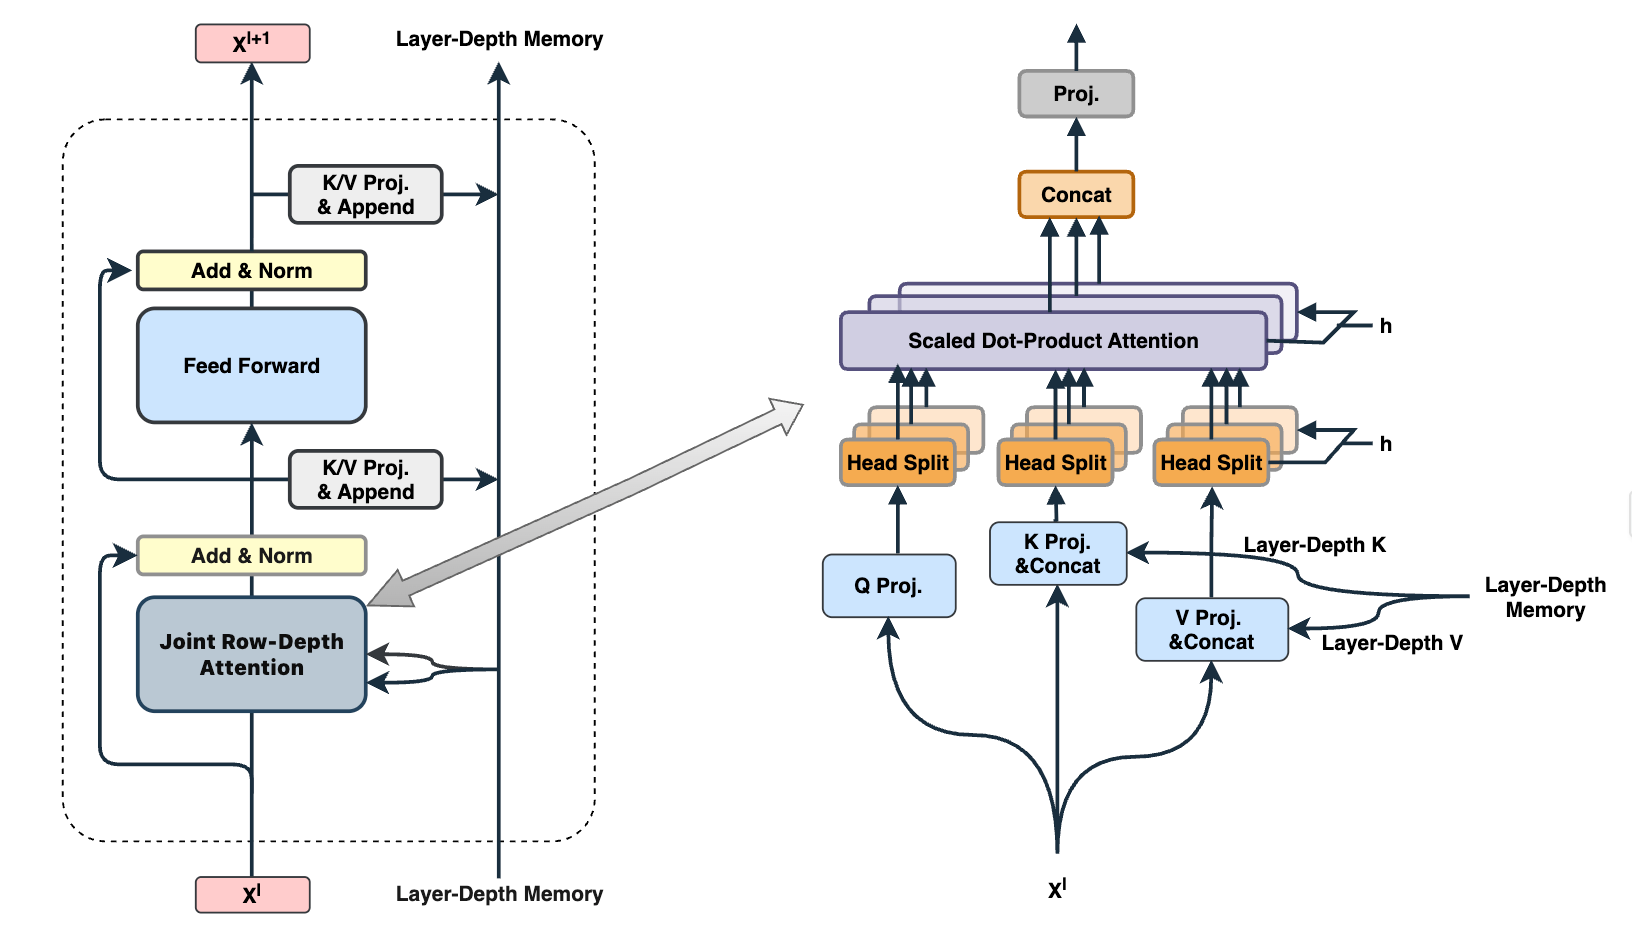
\includegraphics[width=0.95\linewidth]{figures/figure1_architecture.png}
    \caption{Overview of the proposed layer-depth attention routing block. The standard row-wise causal attention pathway is preserved, while the block also exports one projected K/V entry to a layer-depth memory archive. At the next layer, the current token uses a single query to route attention jointly over current-layer token context and earlier-layer same-position memory. Row-wise scores and depth-memory scores are concatenated before a shared softmax, so both sources compete for one unified attention budget.}
    \label{fig:architecture}
\end{figure}

\subsection{Complexity and Memory Overhead}

Let the model have $L$ layers, hidden width $D$, sequence length $S$, batch size $B$, and MLP ratio $r$. A standard decoder-only Transformer has leading-order compute
\[
C_{\text{base}} = L\bigl((4+2r)BSD^2 + 2BS^2D\bigr).
\]
For the commonly used $r=4$ setting, this becomes
\[
C_{\text{base}} = L\bigl(12BSD^2 + 2BS^2D\bigr).
\]

Relative to the baseline, our method changes only two parts of the computation: it adds historical K/V projections for the depth-memory archive, and it expands the attention score tensor from token-only routing to joint row-depth routing. Concretely, the baseline attention block contains $QKV$ projection plus output projection, contributing $4BSD^2$ per layer before the MLP term. In our current implementation, each layer additionally computes one projected memory $K/V$ pair for the historical archive, adding another $2BSD^2$ per layer. This yields a total projection term of $(6+2r)BSD^2$ once the MLP is included. In the same implementation, each layer contributes one historical entry, so the $l$-th layer reads
\[
M_l = l-1
\]
depth-memory slots. Substituting this into the layerwise cost gives the following closed-form model complexity:
\[
C_{\text{method}} \approx L\bigl((6+2r)BSD^2 + 2BS^2D\bigr) + BSD\,L(L-1).
\]
Under the current $r=4$ setting, this becomes
\[
C_{\text{method}} \approx L\bigl(14BSD^2 + 2BS^2D\bigr) + BSD\,L(L-1).
\]

Thus, compared with the baseline, the method introduces an additional $2LBSD^2$ projection term and an additional $BSD\,L(L-1)$ depth-matching term. The main point is that the method adds a moderate but non-negligible amount of work on top of standard self-attention rather than replacing the Transformer computation wholesale.

In memory terms, the relevant quantity in our experiments is training-time peak GPU memory. Relative to the baseline, the proposed method must retain additional historical K/V activations and intermediate depth-branch tensors, which increases training memory usage but does not change the overall order of growth with sequence length in the same dramatic way as introducing another full token-token attention matrix would. Empirically, the measured peak-memory increase is modest compared with the runtime slowdown, suggesting that the current prototype is more constrained by systems-level execution overhead than by raw storage growth alone.

\section{Experiments}

\subsection{Benchmark and Setup}

Our main benchmark is \textbf{WikiText-103} in the raw-text setting \cite{merity2016wikitext}. All experiments use a BPE tokenizer, specifically the GPT-2 tokenizer \cite{radford2019gpt2}, and train decoder-only language models with tied input/output embeddings unless otherwise noted \cite{press2017tie}.

All models in the main comparison use the same decoder-only Transformer backbone family implemented in \texttt{ablation\_models.py}. Unless a specific ablation changes the attention mechanism itself, the backbone remains matched across methods in hidden size, head count, MLP ratio, positional embeddings, and language-model head structure.

The main completed result pool already supports a coherent comparison across multiple settings:
\begin{itemize}[leftmargin=1.5em]
    \item 8-layer, $seq\_len=256$, $40000$ and $80000$ steps;
    \item 16-layer, $seq\_len=256$, $80000$ steps;
    \item 8-layer, $seq\_len=512$, $80000$ steps;
    \item projected-K/V versus non-projected historical K/V.
\end{itemize}
Most runs use $d\_model=384$, $num\_heads=8$, $mlp\_ratio=4$, tied embeddings, and learned positional embeddings. This places the experiments in the same general decoder-only language-modeling regime as prior WikiText-103 Transformer studies \cite{baevski2018adaptive,dai2019transformerxl}.

Validation is performed periodically during training, while the test set is evaluated only at the end of the run. For this reason, we consistently report \textbf{Best Val PPL} and \textbf{Final Test PPL} rather than best test perplexity. Each reported result is the median of three runs under the same configuration; the observed variation is small enough that we do not list a separate variance column in the main table.

\subsection{Main Results}

Across all completed settings, the final \textbf{single-q + projected K/V} method consistently outperforms the standard Transformer baseline in both best validation perplexity and final test perplexity.

In the 8-layer, $seq\_len=256$ setting, the method reduces final test perplexity from $34.53$ to $33.53$ at $40000$ steps, and from $28.47$ to $27.58$ at $80000$ steps. In the 16-layer, $seq\_len=256$ setting, it further reduces final test perplexity from $26.28$ to $25.55$. The gain also persists at longer context length, where the 8-layer, $seq\_len=512$ setting improves from $24.03$ to $23.46$.

Taken together, the currently completed settings show stable relative final-test-perplexity improvements ranging from 1.3\% to 3.1\% across model depth, context length, and training budget. Although the absolute gains are moderate rather than dramatic, they are consistent across all currently completed main settings. For completeness, validation-loss curves for the two main $seq\_len=256$ settings are provided in the appendix.

\begin{table}[t]
    \centering
    \small
    \setlength{\tabcolsep}{4pt}
    \resizebox{\linewidth}{!}{%
    \begin{tabular}{lccccccccc}
        \toprule
        Method & Layers & Seq Len & Steps & Params (M) & Best Val PPL & Final Test PPL & Step Time (s) & Tokens/s & Peak GPU Mem (GB) \\
        \midrule
        Baseline & 8  & 256 & 40000 & 33.59 & 33.55 & 34.53 &  &  &  \\
        Ours     & 8  & 256 & 40000 & 33.89 & 32.37 & 33.53 &  &  &  \\
        Baseline & 8  & 256 & 80000 & 33.59 & 27.58 & 28.47 & 0.0826 & 24793.0 & 7.81 \\
        Ours     & 8  & 256 & 80000 & 33.89 & 26.51 & 27.58 & 0.1027 & 19939.0 & 8.44 \\
        Baseline & 16 & 256 & 80000 & 47.80 & 25.29 & 26.28 & 0.1263 & 16210.1 & 9.58 \\
        Ours     & 16 & 256 & 80000 & 48.08 & 24.63 & 25.54 & 0.2272 & 9014.0 & 9.60 \\
        Baseline & 8  & 512 & 80000 & 33.69 & 23.53 & 24.02 & 0.1910 & 21446.5 & 11.23 \\
        Ours     & 8  & 512 & 80000 & 33.99 & 22.89 & 23.46 & 0.2462 & 16638.2 & 10.82 \\
        Baseline & 16 & 512 & 80000 & 47.80 & 21.87 & 21.37 & 0.3120 & 13126.1 & 12.27 \\
        Ours     & 16 & 512 & 80000 & 48.08 & 20.51 & 21.09 & 0.3869 & 10587.0 & 13.51 \\
        \bottomrule
    \end{tabular}
    }
    \caption{Main WikiText-103 results and cost-performance comparison. Each entry reports the median of three runs under the same configuration. The proposed method consistently improves validation and test perplexity across the completed settings with nearly unchanged parameter count. For the 80{,}000-step runs, step time, throughput, and peak GPU memory are reported under matched training configurations.}
    \label{tab:main-results}
\end{table}

\subsection{Attention Allocation and Retrieval Patterns}

Beyond perplexity, the attention analyses provide direct evidence that the added depth branch is functionally active rather than a passive architectural perturbation. The most basic statistic is the average attention mass assigned to the row branch versus the depth branch. In the 16-layer model, early layers remain dominated by row-wise token attention, but middle and late layers allocate substantially more mass to depth retrieval; in the deepest layers, the average depth mass becomes comparable to or slightly larger than the row mass, as shown in \Cref{fig:row-depth-mass}.

This raw layer-wise increase must be interpreted carefully. Deeper layers also expose more memory slots, so part of the increase in total depth mass is structurally induced by a larger candidate set. We therefore also inspect slot-normalized views and the depth-slot heatmap. These show that the growth in total depth usage is only partly explained by slot count: even after accounting for the number of available historical slots, middle and late layers still retain nontrivial per-slot depth usage. More importantly, the slot-allocation heatmap shows that the model does not distribute attention uniformly over all available history. Instead, it exhibits a marked preference for a small set of early memory slots, especially those near the bottom of the network.

\begin{figure}[t]
    \centering
    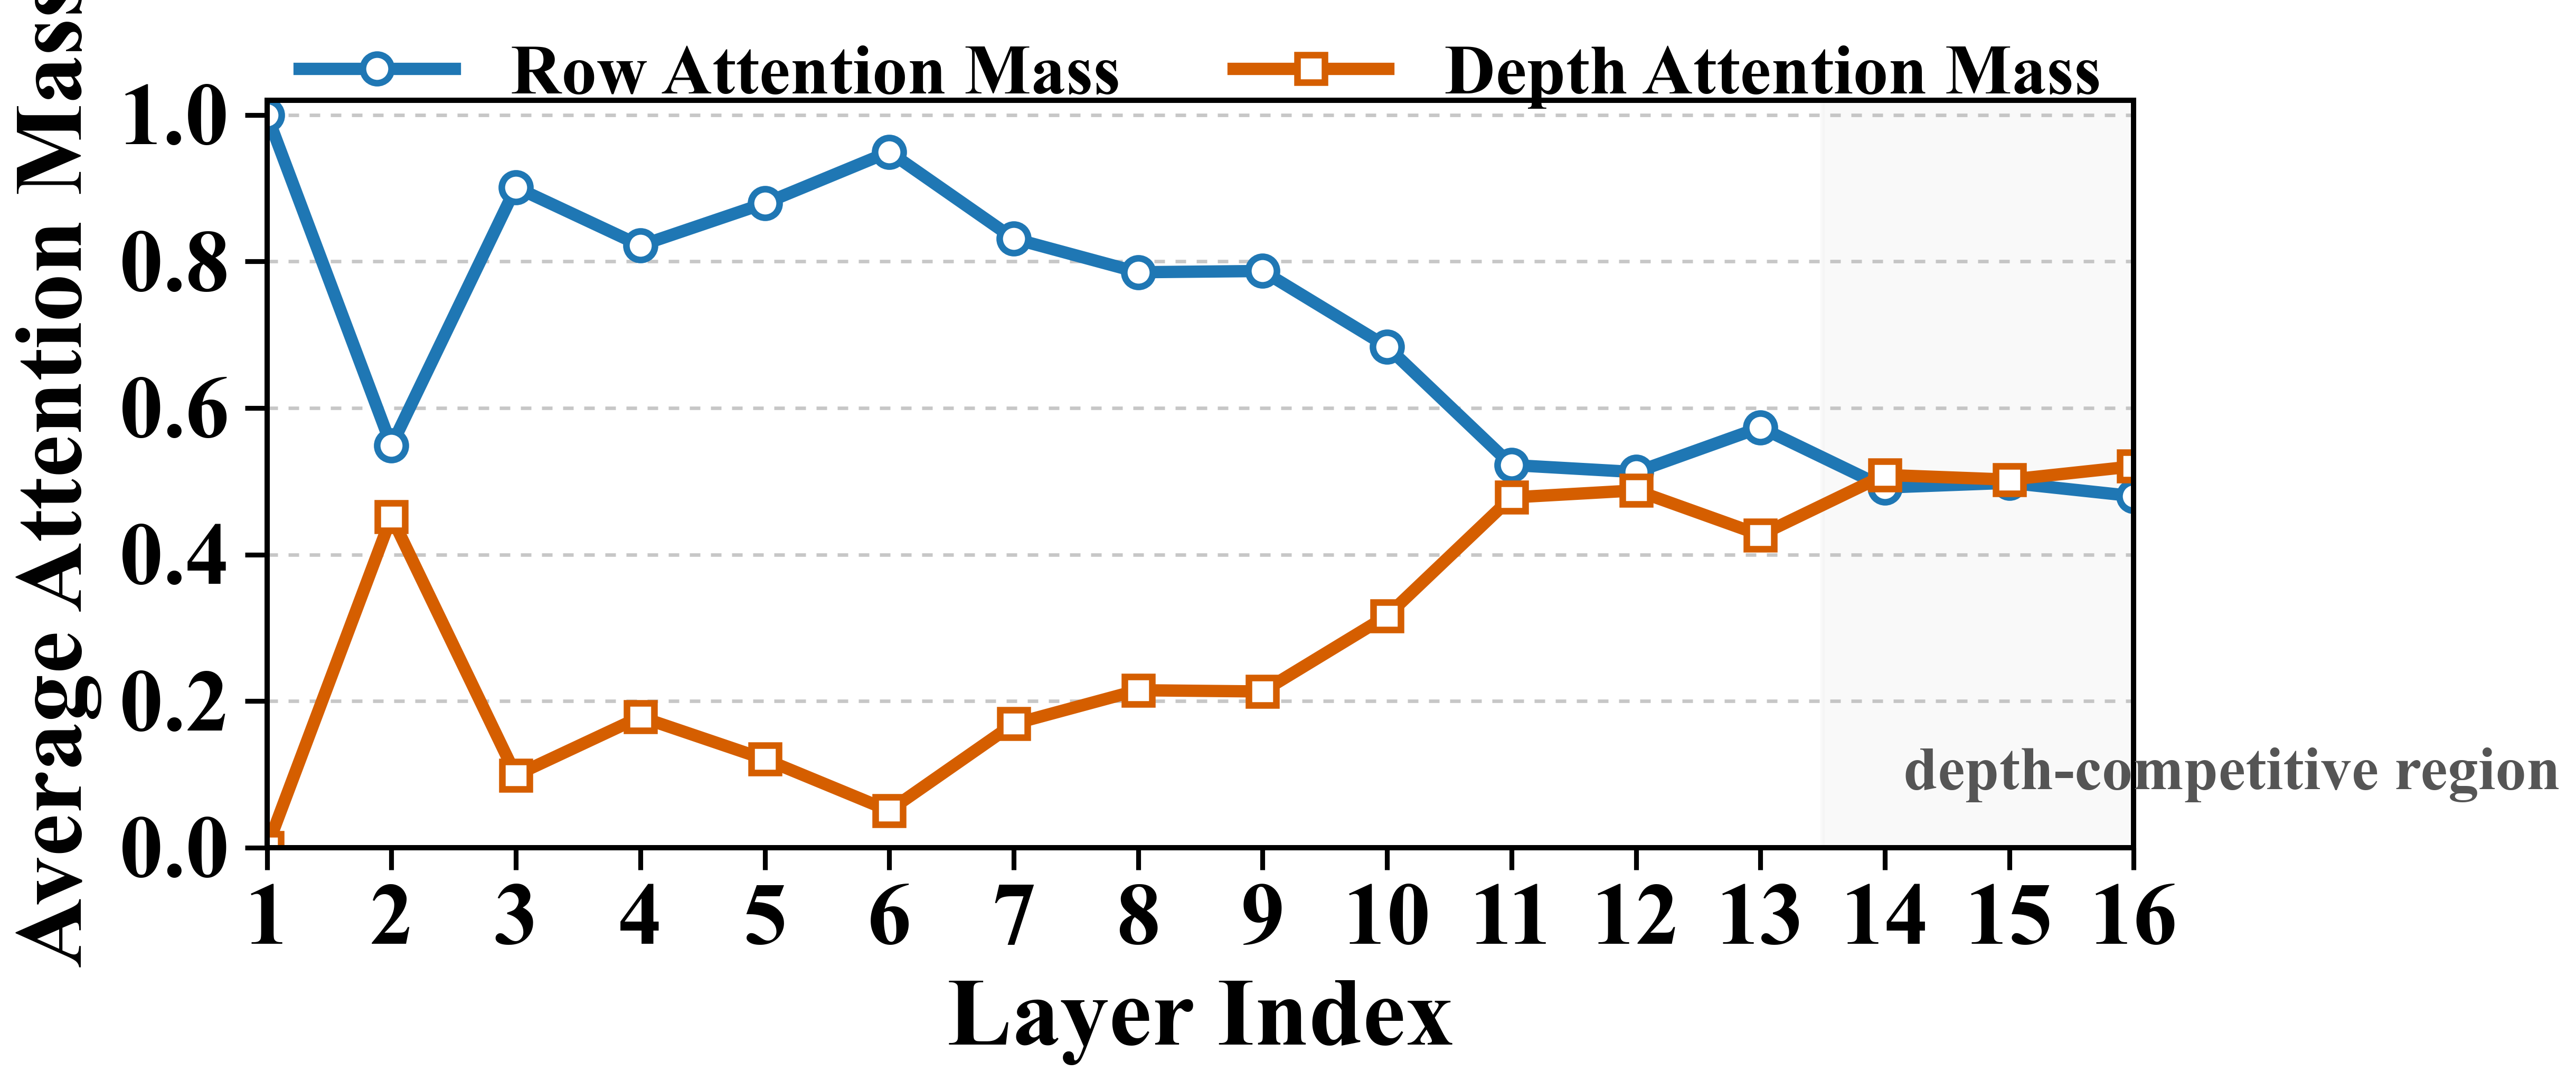
\includegraphics[width=0.78\linewidth]{figures/figure3f_row_vs_depth_mass_by_layer.png}
    \caption{Average row-vs-depth attention mass by layer for the 16-layer model. Early layers remain strongly row-dominated, while middle and late layers allocate progressively more attention mass to the depth branch. In the deepest layers, depth retrieval becomes competitive with or slightly stronger than row-wise token routing.}
    \label{fig:row-depth-mass}
\end{figure}

This trend becomes more informative when combined with the token-position analysis in \Cref{fig:depth-by-position}. The depth branch grows stronger as layer depth increases, but does not collapse into a narrow set of late-sequence positions. After excluding the earliest positions where the available token context is still very small, the depth-share pattern remains broadly stable across token positions. Intuitively, the row branch gains access to more token candidates as the sequence position increases, yet the model does not simply reallocate its entire budget toward the token axis. This suggests that depth retrieval remains functionally relevant even when the token branch has many more available competitors.

Together with the joint-attention matrices, these observations support a more specific interpretation of the mechanism. The depth branch is not only active in deeper layers; it also tends to place substantial weight on a small number of early historical entries. In the current model, these entries correspond to very early layer states, close to the bottom of the network. This indicates that the proposed architecture gives deeper layers a more direct path to low-level or lightly transformed representations. Standard residual connections also propagate such information forward, but the present results suggest that residual mixing alone may be insufficient for strong and selective reuse of those early-layer signals.

\begin{figure}[t]
    \centering
    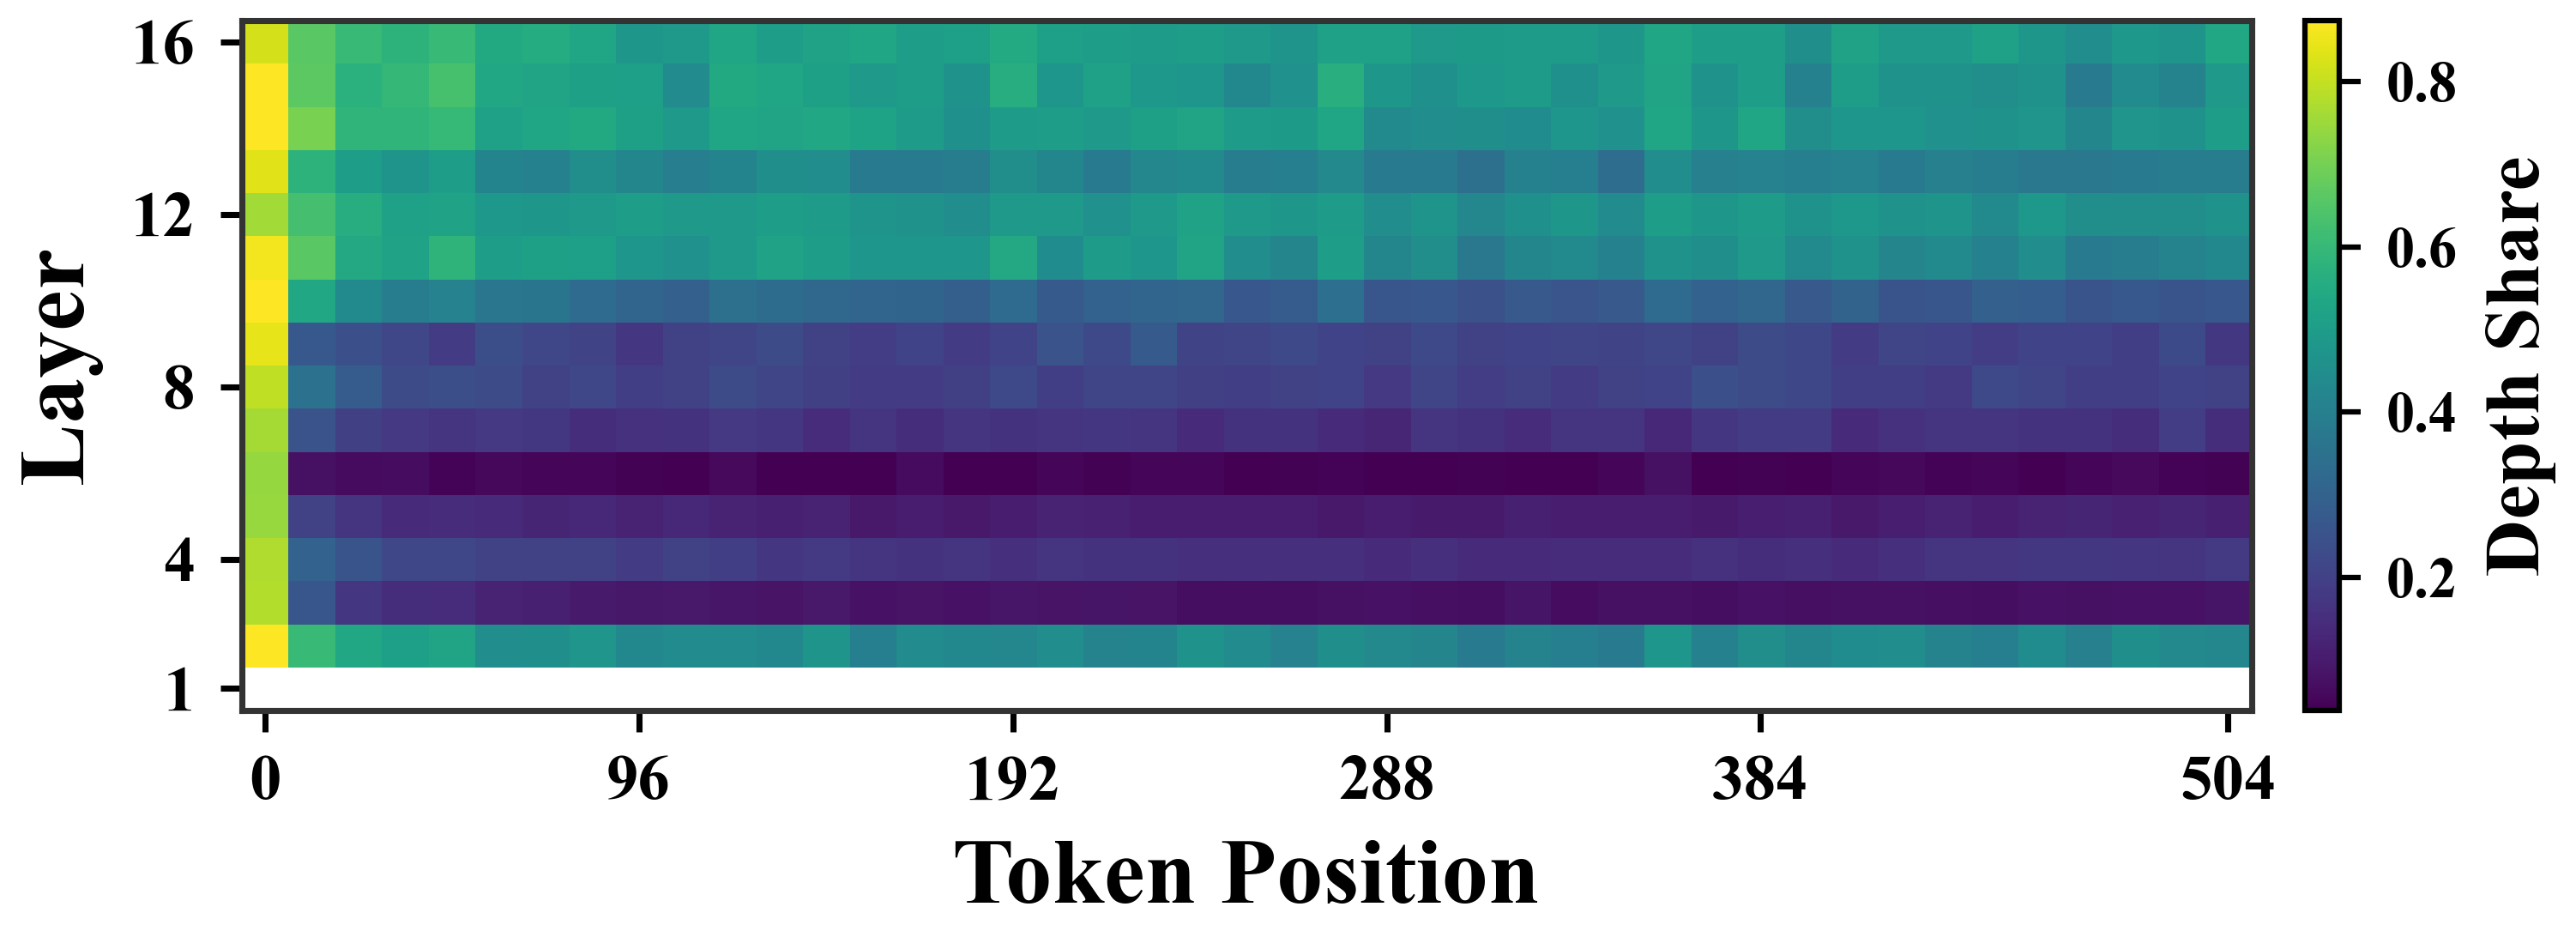
\includegraphics[width=0.74\linewidth]{figures/figure3g_depth_attention_share_sampled_s12_flat_v4.png}
    \caption{Depth-attention share as a function of layer and token position in the 16-layer model. The horizontal axis is sampled every 12 positions for readability. The dominant variation is across layer depth rather than token position: depth retrieval becomes markedly stronger in middle and late layers, while remaining broadly stable across most token positions once the very earliest prefix region is excluded.}
    \label{fig:depth-by-position}
\end{figure}

The single-example attention matrices in \Cref{fig:attention-analysis} clarify the qualitative difference between the baseline and the proposed method. In the baseline, the entire attention budget is distributed over token positions only. In the proposed model, the row branch is preserved, but the joint matrix additionally assigns visible mass to a separate region of depth slots. This makes the final attention pattern more selective: the model is no longer limited to distributing mass across token positions alone, and instead routes part of the budget toward a small number of high-value historical states.

These observations do not by themselves prove improved scaling to larger models or much longer training runs. However, they do provide encouraging evidence in that direction. The depth branch does not fade away as layers deepen or as more token candidates become available; instead, it remains active and in some cases becomes more prominent. This is at least consistent with the hypothesis that explicit layer-depth retrieval remains useful under deeper architectures and longer-context settings.

\begin{figure}[t]
    \centering
    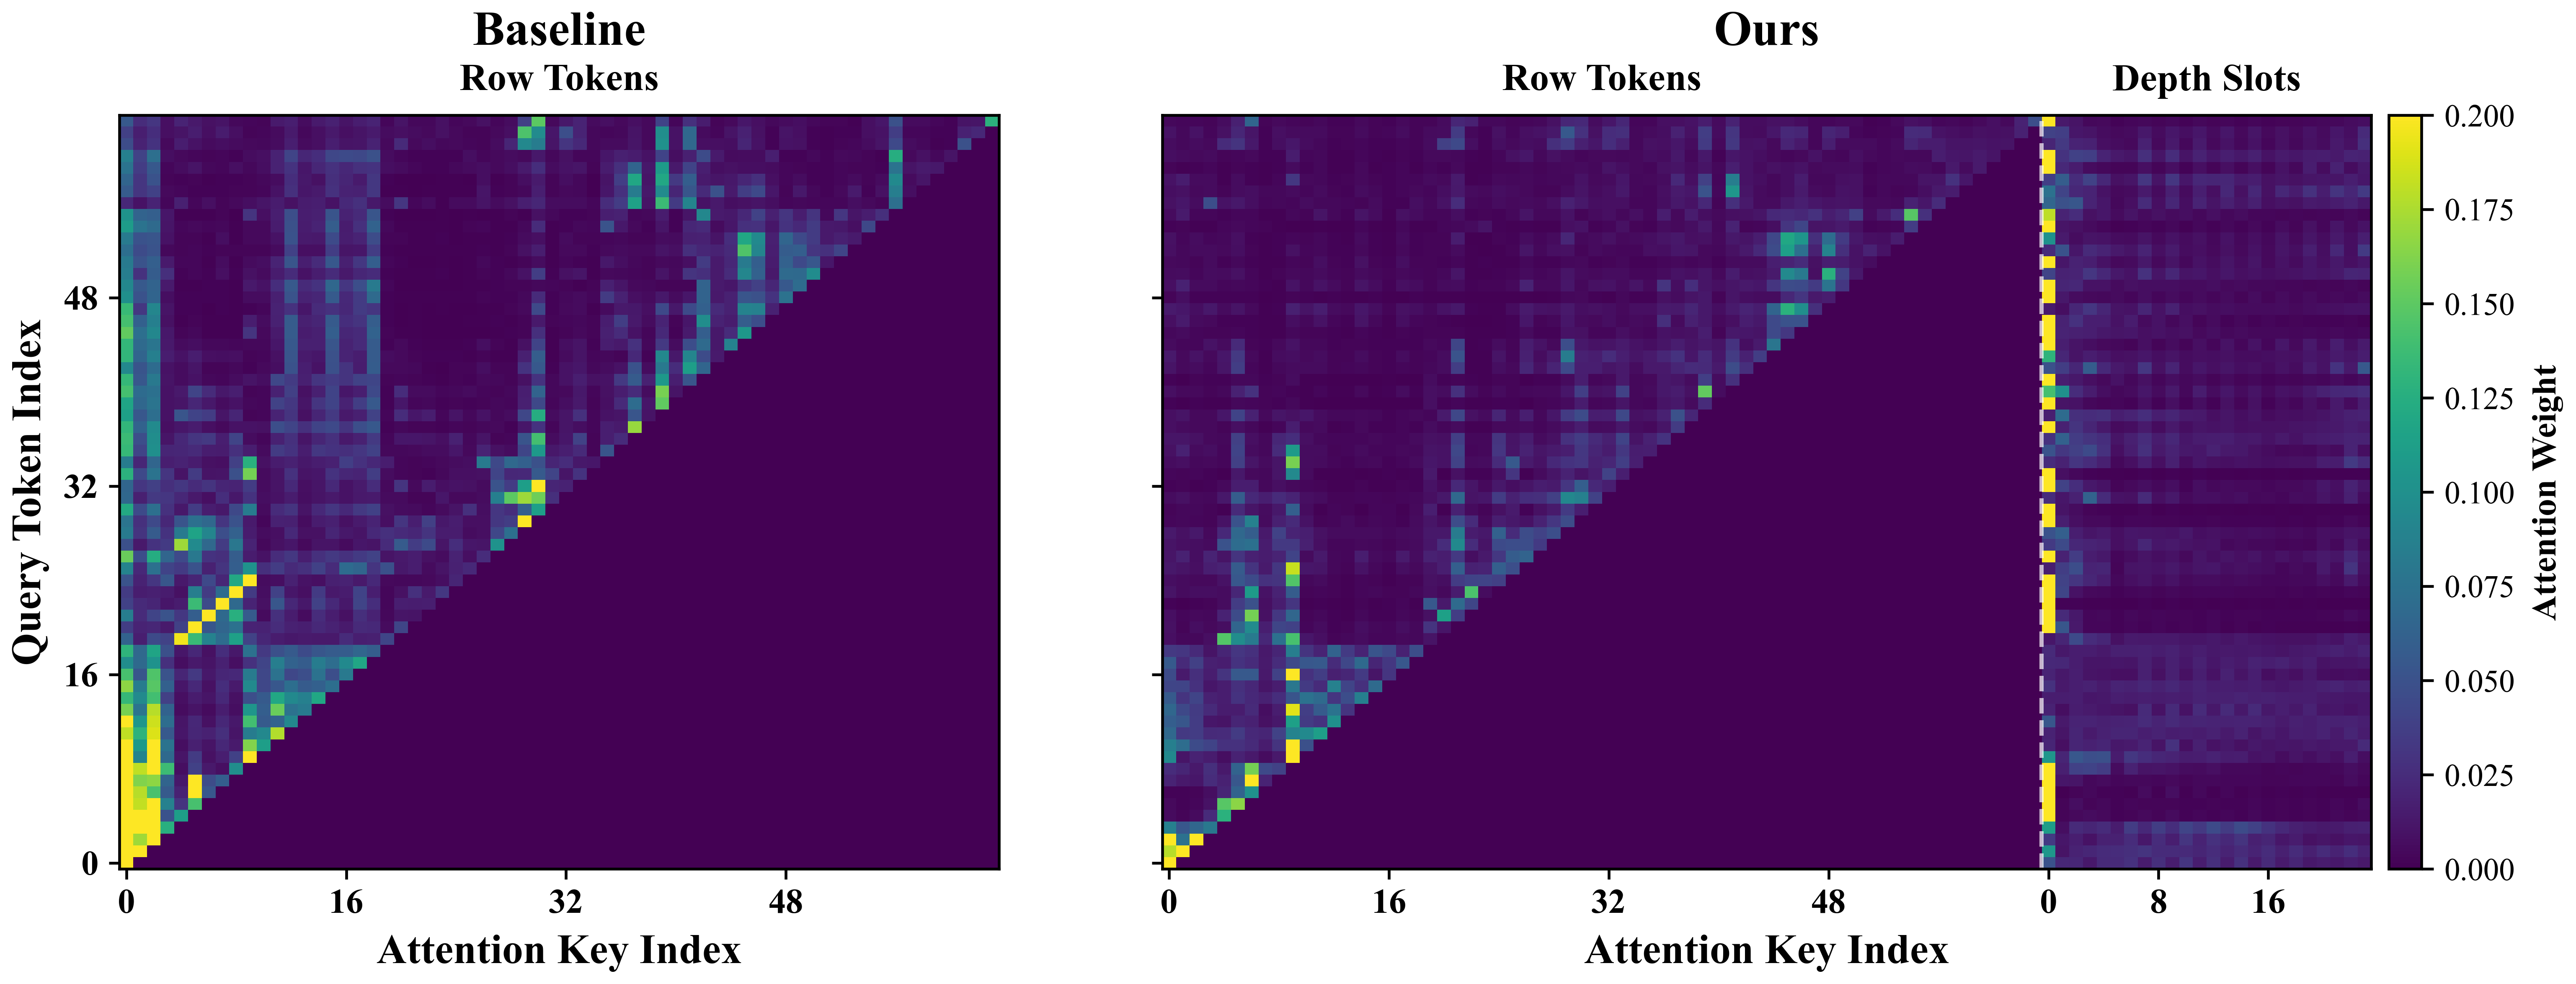
\includegraphics[width=0.92\linewidth]{figures/figure3e_joint_attention_baseline_vs_ours_final.png}
    \caption{Joint attention maps at layer 13 with sequence length 64. In the baseline, the attention budget is distributed entirely over token positions. In the proposed model, the row-token pathway is preserved but a distinct depth-slot region also receives visible attention mass. This shows that the model does not ignore the added branch; instead, it allocates part of the joint attention budget to a compact set of high-value layer-depth memory slots.}
    \label{fig:attention-analysis}
\end{figure}

\subsection{Ablation Summary}

The current ablation evidence indicates that the overall layer-depth routing idea is robust, while the best parameterization of the memory branch remains an open empirical question. In particular, the final single-query projected-K/V design is clearly better than the baseline, but not every accompanying design decision contributes equally. For context, we also include an Attention Residuals-style comparison method under the same training stack.

\begin{table}[t]
    \centering
    \small
    \setlength{\tabcolsep}{5pt}
    \resizebox{\linewidth}{!}{%
    \begin{tabular}{lcccccccc}
        \toprule
        Variant & Layers & Seq Len & Steps & Params (M) & Best Val PPL & Final Test PPL & Rel. Gain & Notes \\
        \midrule
        Baseline & 8 & 256 & 80000 & 33.59 & 27.58 & 28.47 & 0.00\% & reference \\
        Ours (single-q + projected K/V) & 8 & 256 & 80000 & 33.89 & 26.51 & 27.58 & 3.12\% & final method \\
        Ours w/o sublayer & 8 & 256 & 80000 & 33.89 & 26.77 & 27.81 & 2.31\% & block memory \\
        Ours w/o projected K/V & 8 & 256 & 80000 & 33.59 & 27.06 & 28.12 & 1.23\% & raw-history variant \\
        Attention Residuals & 8 & 256 & 80000 &33.60  & 33.47 & 32.57 & -- & related baseline \\
        \bottomrule
    \end{tabular}
    }
    \caption{Key ablation summary on the core 8-layer, sequence-length-256 setting. The final single-query projected-K/V design gives the strongest core result among the completed variants currently considered in the paper.}
    \label{tab:ablation}
\end{table}

\section{Related Work}

Modern decoder-only language models are built around causal self-attention over the token dimension \cite{vaswani2017attention,radford2019gpt2}. This design has proved extremely effective, and prior work has long emphasized that one of its key benefits is the drastic reduction of communication path length along the sequence axis compared with recurrent architectures \cite{vaswani2017attention}. Our work starts from the observation that this leaves a complementary axis underused, namely the depth history of the same token across previous layers \cite{zhang2026residual}.

A broad family of prior work has explored augmenting Transformers with memory mechanisms, recurrent state, cached history, or cross-layer interactions. Some methods enlarge the effective context window by storing additional information across segments or decoding steps, as in Transformer-XL \cite{dai2019transformerxl}; others revisit how repeated computation itself should be organized, as in Universal Transformer \cite{dehghani2018universal}; still others modify how information from different depths is reused through learned cross-layer aggregation or depth-wise routing \cite{ravula2021realformer,denseformer2024,dca2025,muddformer2025,kimi2026attnres}. Our method belongs most naturally to this last category, but with a narrower design goal: enabling a token at the current layer to retrieve its own same-position history from earlier layers.

Another nearby line of work asks whether standard residual propagation can be improved by learned aggregation across layers or modified residual-attention pathways \cite{ravula2021realformer,denseformer2024,dca2025,kimi2026attnres}. These methods are highly relevant to our motivation, since they likewise recognize that useful information may be distributed across depth rather than only along the current layer's token axis. However, our approach preserves the standard token-attention branch and organizes retrieval around same-position historical memory entries, rather than treating the entire layer stack as a generic pool for residual recombination. In this sense, it is also closely related to recent attempts to explicitly factor Transformer information flow into sequence and depth axes \cite{zhang2026residual}, while remaining complementary to depth-stabilization methods such as DeepNet \cite{wang2022deepnet}. Parameter-sharing work such as ALBERT \cite{lan2019albert} is also tangentially relevant, because it highlights that what matters across depth is not merely stacking more layers, but how information and computation are reused across them. Our method addresses that question from the retrieval side rather than from the parameter-sharing side.

\section{Conclusion}

This paper studies a simple architectural question: can a decoder-only Transformer benefit from explicitly reading the same token's depth history, rather than relying only on residual propagation through the layer stack? The experiments presented here suggest that the answer is yes. Across the completed WikiText-103 settings, a layer-depth memory routing mechanism yields stable perplexity improvements over standard Transformer baselines across multiple depths, sequence lengths, and training budgets.

The main empirical message is not that the gains are dramatic, but that they are repeatable. This is important because the baseline models used here are already reasonably strong, and therefore the observed 1.3\% to 3.1\% improvements in final test perplexity are better interpreted as stable architectural gains than as artifacts of a weak comparison point.

At the same time, the work also exposes a clear trade-off. The current prototype incurs noticeable runtime overhead, and the measured slowdown is larger than the pure analytical compute increase. This indicates that the present implementation should still be viewed as an early but credible systems prototype rather than a fully optimized final design.

The broader conclusion is that depth history is a real information source for decoder-only language models. A token does not only need access to earlier tokens; it can also benefit from direct access to what earlier layers already computed at the same position. The accompanying attention analyses support this interpretation: the trained model assigns substantial mass to the depth branch in deeper layers and concentrates retrieval on a small number of high-value historical slots rather than ignoring the branch or averaging uniformly over history. The proposed layer-depth routing mechanism provides one concrete way to expose that signal. Future work should clarify the best memory parametrization, improve runtime efficiency, and test whether the same design principle carries to larger models and broader language-model settings.

\appendix

\section{Appendix: Default Experimental Settings}

\begin{table}[t]
    \centering
    \small
    \setlength{\tabcolsep}{6pt}
    \begin{tabular}{ll}
        \toprule
        Hyperparameter / Option & Default Value \\
        \midrule
        Dataset & WikiText-103 raw \\
        Tokenizer & GPT-2 BPE \\
        Sequence length & 256 \\
        Hidden width $D$ & 384 \\
        Layers $L$ & 8 \\
        Attention heads & 8 \\
        MLP ratio $r$ & 4 \\
        Dropout & 0.1 \\
        Tied input/output embeddings & On \\
        Positional embeddings & On \\
        Batch size & 8 \\
        Gradient accumulation steps & 1 \\
        Training steps & 40{,}000 \\
        Evaluation interval & 1{,}000 steps \\
        Evaluation batches & 100 \\
        Learning rate & $3\times 10^{-4}$ \\
        Minimum LR scale & 0.1 \\
        Warmup steps & 100 \\
        Weight decay & 0.01 \\
        Gradient clipping & 1.0 \\
        Random seed & 42 \\
        \bottomrule
    \end{tabular}
    \caption{Default training configuration used by the WikiText ablation script. Main-paper comparisons override only the fields explicitly shown in the result tables, most notably layer count, sequence length, and total training steps.}
    \label{tab:default-settings}
\end{table}

\section{Appendix: Training Curves}

\begin{figure}[t]
    \centering
    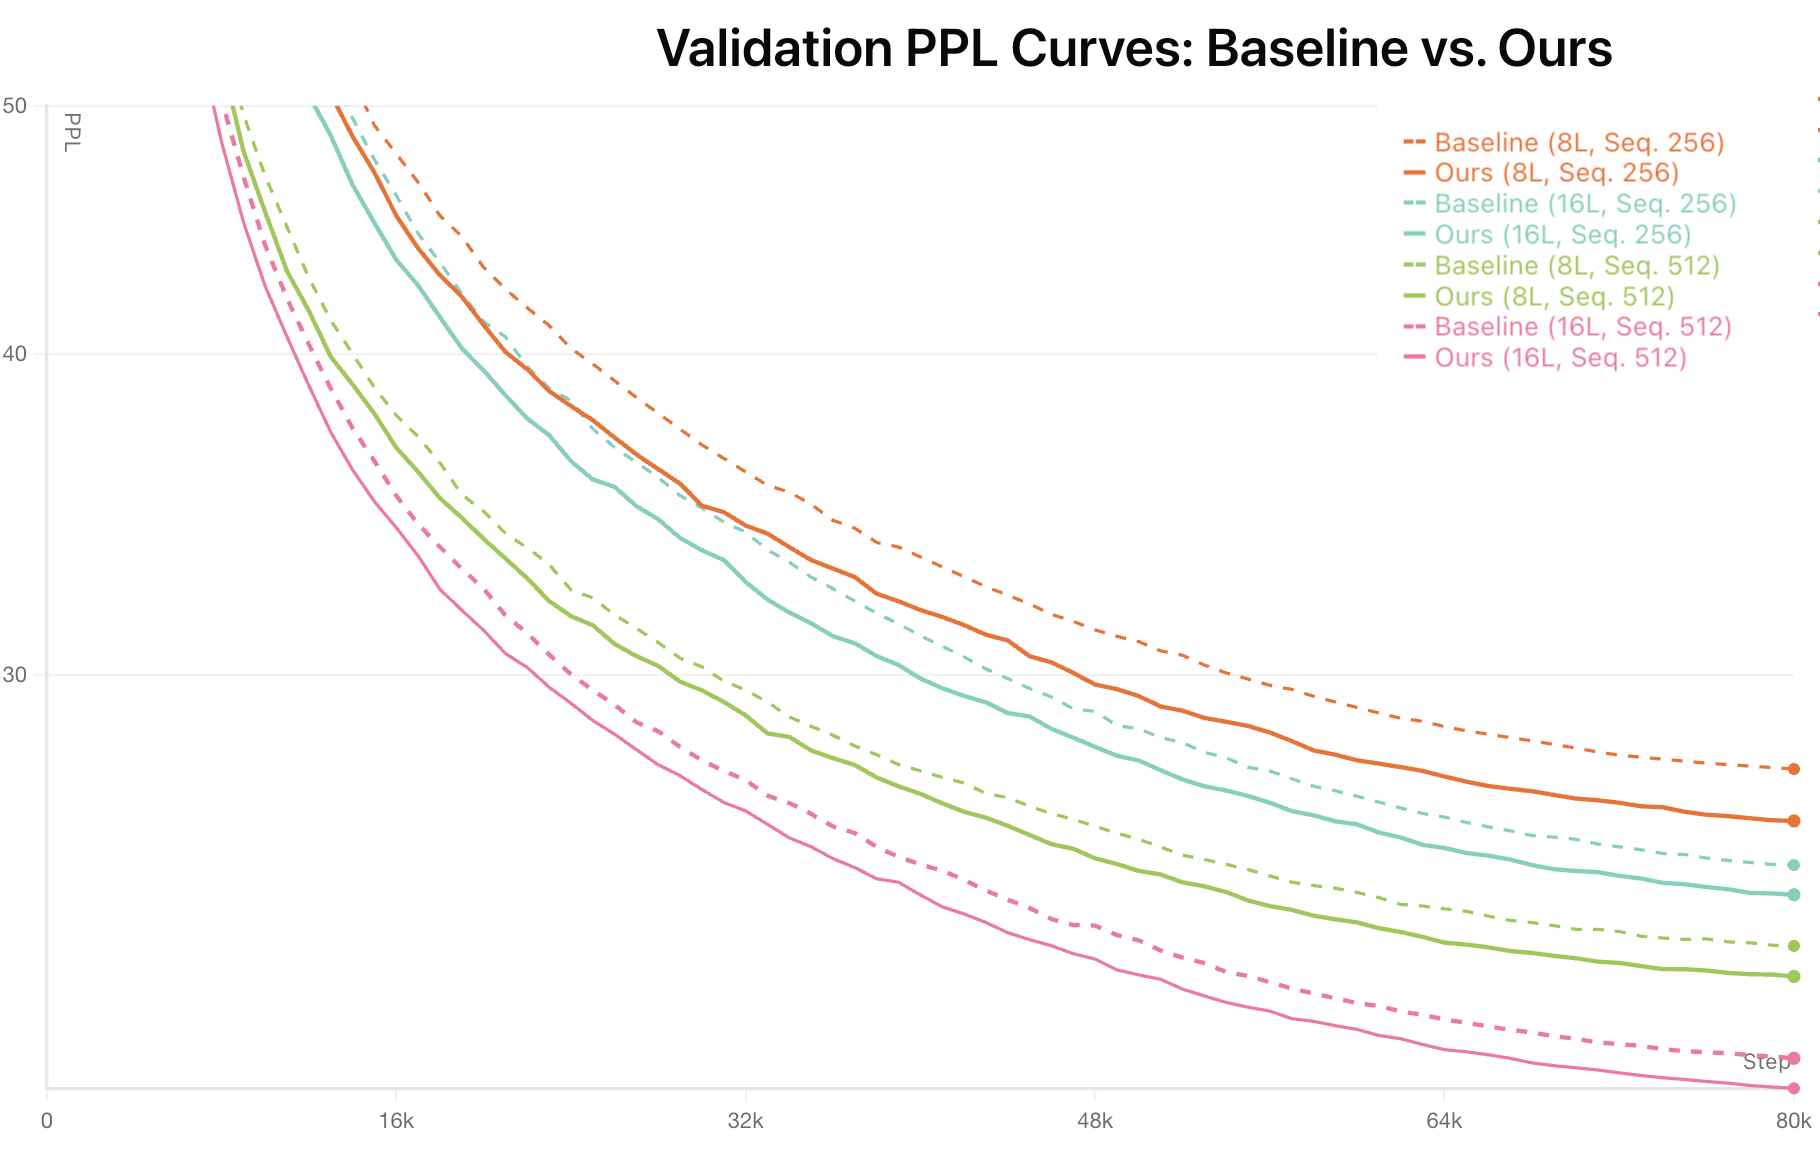
\includegraphics[width=0.88\linewidth]{figures/figure2_training_curves.png}
    \caption{Validation-loss curves for the main WikiText-103 comparisons at sequence length 256. Solid lines denote the proposed method and dashed lines denote the baseline; colors distinguish the 8-layer and 16-layer settings. The proposed method remains competitive early and retains lower validation loss than the baseline over the main completed training ranges.}
    \label{fig:training-curves}
\end{figure}

\clearpage
\bibliographystyle{plain}
\bibliography{refs}

\end{document}
